\chapter{Conclusions}\label{cha:conclusion}
% important to relate to the Purpose

% Sätt av ett kort kapitel sist i rapporten till att avrunda och föreslå rikningar för framtida utveckling av arbetet.

In response to the research questions questions, the master thesis has: %investigate if the work can:

\subsubsection{Contributed to the domain of entrepreneurship education in a developing country context}
This research shows that an app can be effectively used during and after training to assess and learn entrepreneurship. Furthermore, the app can also prepare coaches before youth sessions, training them both in entrepreneurship and preparing their lessons.

In \textit{addition}, this has been done in a developing country context, with coaches having no prior smartphone experience. The app is used for coaches in conjunction with a physical entrepreneurship training today, and does not yet address the youth themselves, or replaces the physical training.

However, the research shows that both the teacher and the coaches greatly appreciates the support the app has given them. As entrepreneurship to its nature is practical in many aspects, one finding is how multiple-choice questions can still simulate real learning, by design solutions such as asking "Are you sure?", giving personal feedback, and formulating questions as scenarios.

\subsubsection{Demonstrated how certain technical constraints and design constraints can be overcome in a developing world context} % service design in development environments % Designprocessen, frågeställning 1

\todo{Lägg till conclusion för denna}

\subsubsection{Provided methods of investigating usability and learnings with a digital training tool in the real-world training context} % Utvärdering, frågeställning 2

To investigate usability, observations using think-aloud in the real-world training context proved the most effective. In big groups, data could give tendencies on common problems that needed to be adressed. In smaller groups, ideas and precise feedback was more common. It helped having a framework to compare usability against, in this case the interaction design principles of desirability, utility, usability and pleasurability.

To investigate learning in the real-world training context, literature research and data analysis of quiz results was highly beneficial, but mostly when put into the context of the observations made in the real-world training context.

Surprisingly often, comparing research and expert opinions with what coaches thought was best for learning, was in unison. When this happens, the self-confidence of the designer can increase, and the designer can be more daring and experimental.

Having much testing and co-creation was a very rewarding approach. To make it truly testable, lo-fi and hi-fi prototypes should be used instead of hypothetical questions. While research before starting to develop is a great start, it was trying different solutions, all based on user advice, expert opinion and research, that gave great results.

\subsubsection{Created new methods in service design, when co-designing digital artefacts in a developing country context}
Short iterations is a challenge, especially when time is sparse and the culture is different than one's own. Often in projects, testing is overlooked. In this project instead, service design helped to look at the users as not only testers, but as co-creators. This is not new in itself, but the creation of Digital Service Design, and methods within this discipline, were new. Examples include sevice mini-sprints and field hackathons.

Interactions with the coaches always included Service Mini-Sprints (see \ref{mini-sprint}), allowing the most important feedback and insights to be addressed in the app and workshop formats already the next day. This allowed for very effective use of the sparse interactions with the coaches, and there was no need to wait for the next iteration to test the coaches' feedback.

The "field hackathon", in which the app was refined and tested each day of the coach training, was the most important piece of the whole master thesis. More than the opportunity to develop the app with the coaches, it had the extra benefit of giving the opportunity to observe the YoungDrive training and understand the coaches.

To use a service design approach when co-creating digital artefacts in a developing country context proved highly effective, and it is recommended that this are is further studied. It does demand bravery of the designer to get to know the users so well, and design for their needs and dare to question the client, but in the end, as in this case, both the users and the client may end up more satisfied with the result.

\section{Future Work}

The future work section is divided by research question, and proposes additions that would strengthen the app goals (see \ref{purpose}).

\subsection{Research question 1}
\section{How is the Development Affected by the Technical Possibilities?}\label{rq1}

Some of the wished development were too complex to be implemented during the master thesis. Below, it is described what future work is wished in the area.

\subsection{Data Analysis Improvements}
Today, data analysis of quiz results takes a tremendous amount of time, and is not easily accessible or understood by the stakeholders. The data needs to be acquired into Google Sheets, and then needs to be enhanced in several ways to be filterable and visualized. The raw data when inserted into Google Sheets can be seen in figure \ref{unprocessedData}.

\begin{figure}[h]
  \centering
  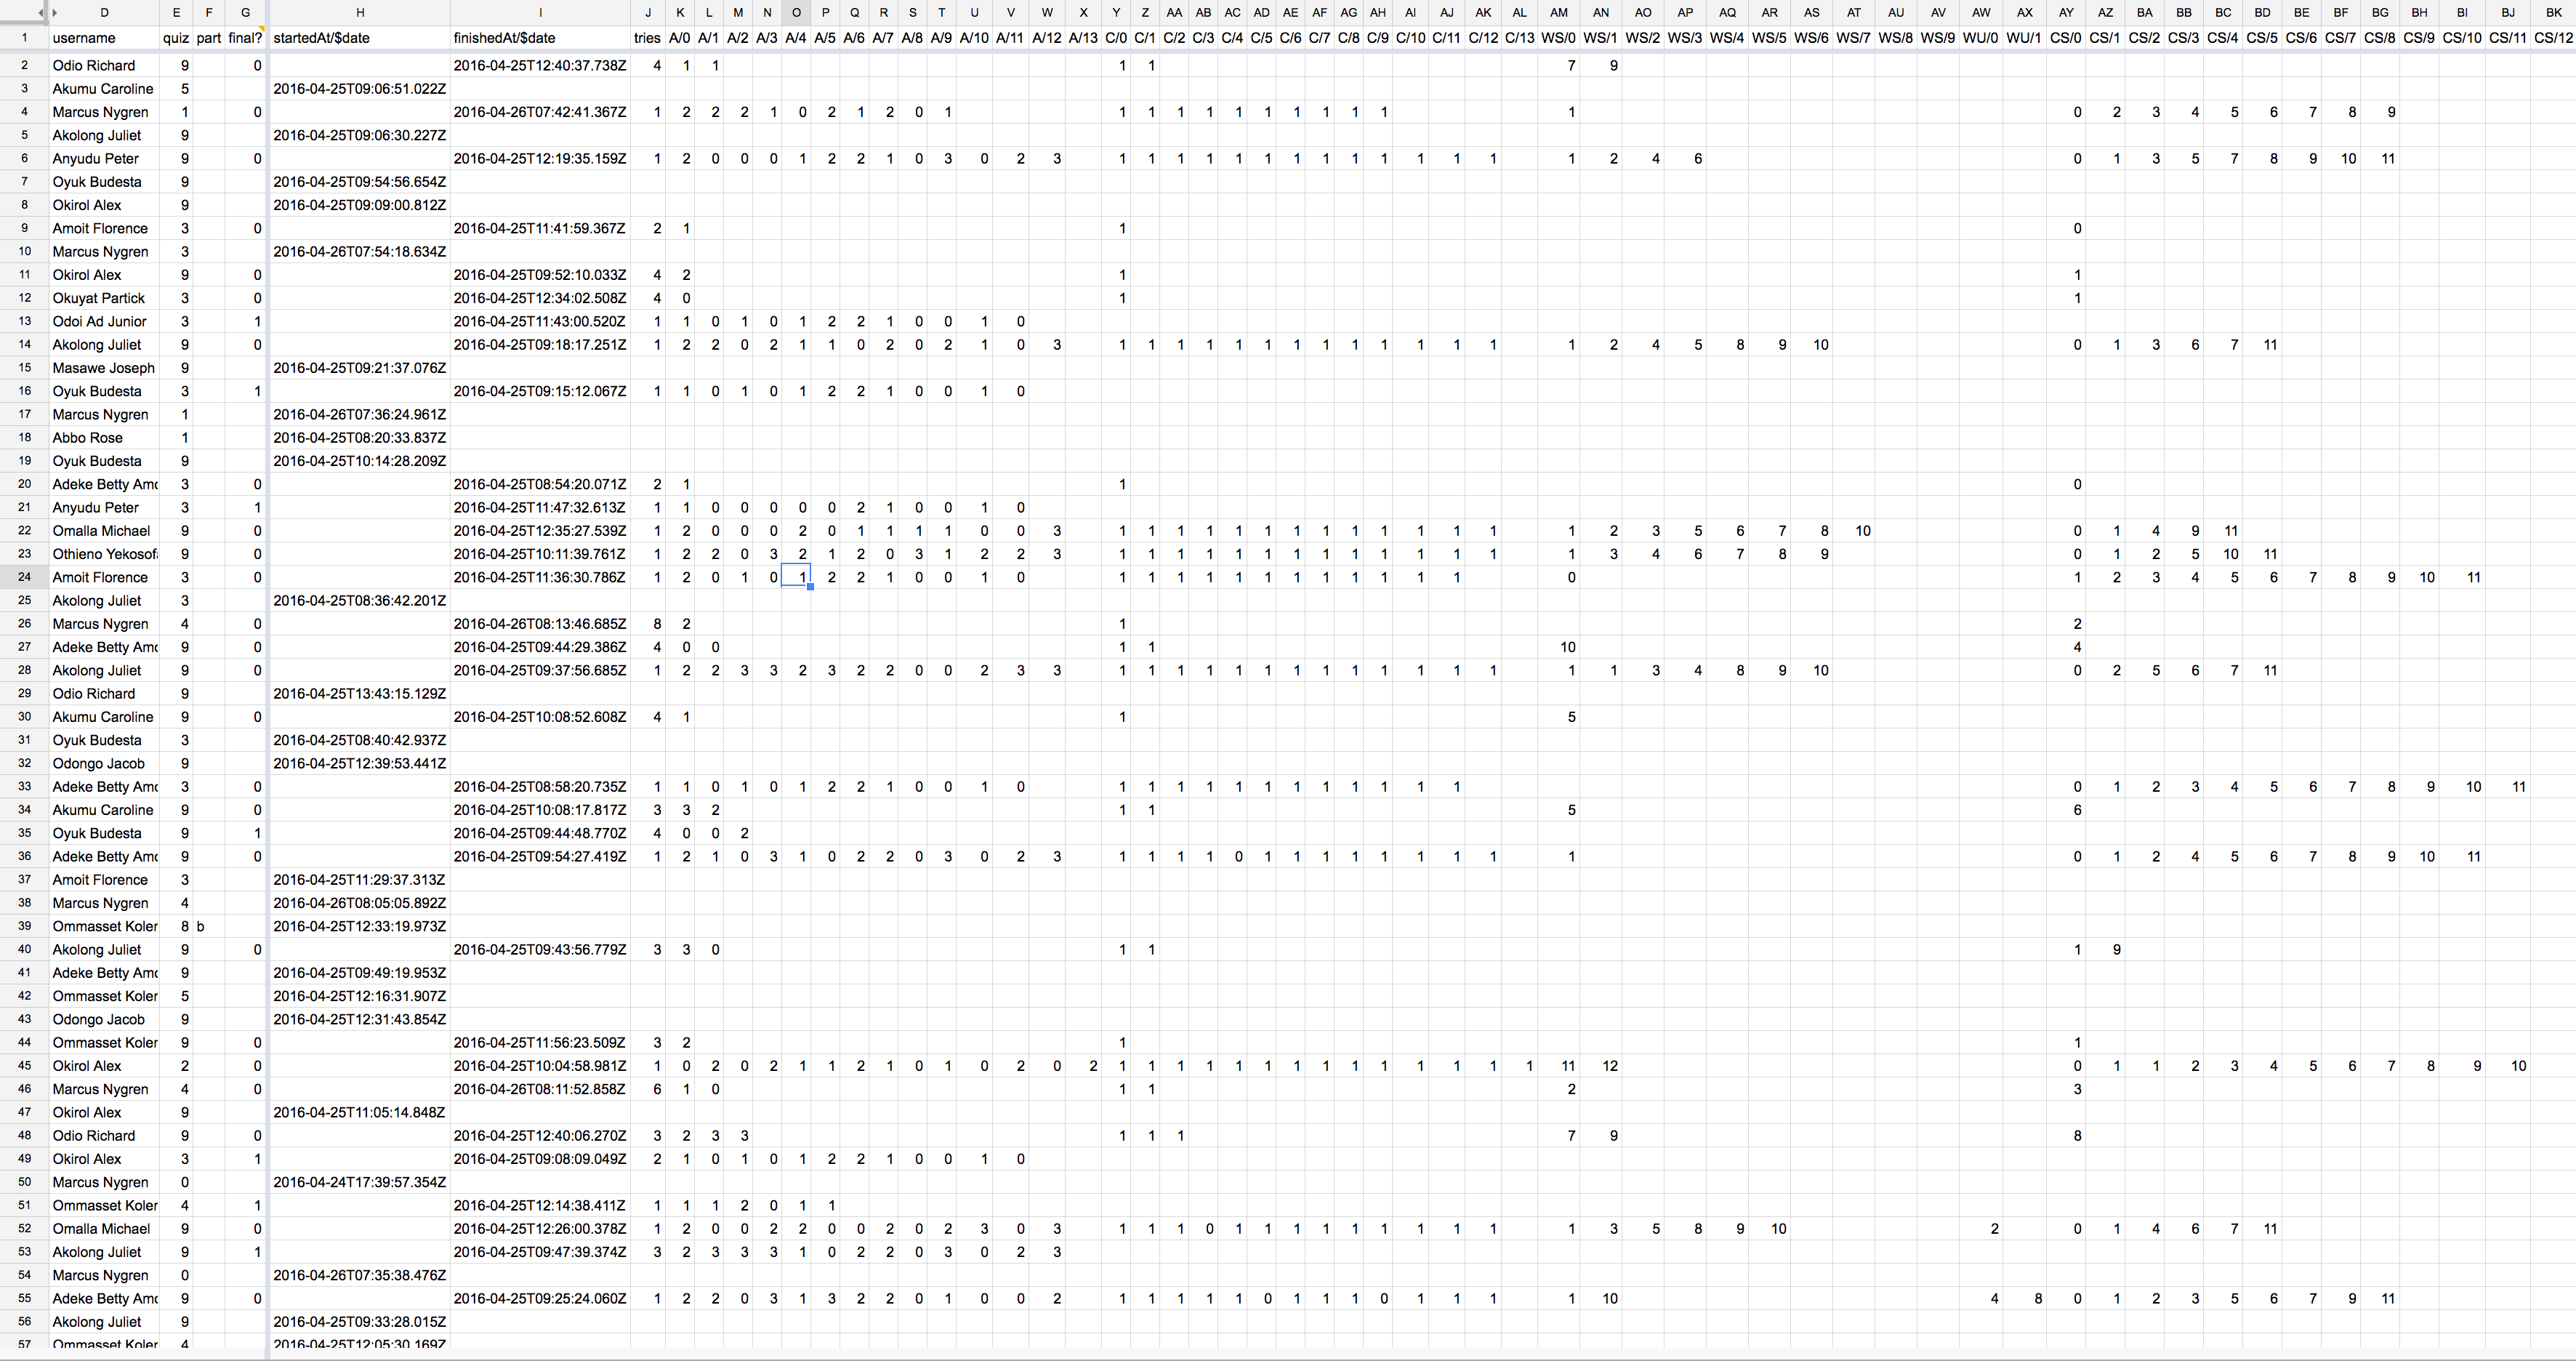
\includegraphics[width=0.8\textwidth]{analysis/unprocessedData.png}
  \caption{The raw data of the quiz results when inserted into Google Sheets.}
  \label{fig:unprocessedData}
\end{figure}

A lot of future development time should be spent so that most of this work is made automatically. Some of this work, is related to the way that the data is saved. Today, whether the coach was correct or incorrect on a question, and how many coaches answered that question incorrect after the first try, needs to be done by process of elimination, because the data is not properly structured in the database.

There were also a small number of errors with quiz submissions in iteration 4. Most notably, certification tests for coach quiz 9 were not submitted, which is why the paper submissions proved very valuable as a backup. To discover more errors regarding offline-online functionality, is important, as it is cumbersome and time-costly to test these manually. A good way to discover such errors, would be automatic tests (or regression tests), so that the app can be used by the coaches with confidence, without extra personnel present, checking that the app works.

\subsection{Code Quality}
Since the app will be continually used and developed by others in the future, code quality is important. React.js makes it easy to structure the code in a way that gives a new developer a good overview of the different components, and its functionality. Even so, refactoring the code into smaller components would be a good idea.

To increase speed of the app, refactoring the code to ensure that loading of assets happen more effectively (especially quiz questions), and also that data is cached in a logical way (saving neccessary information so that it does not need to load the same information again, and vice versa), would be helpful.

As the YoungDrive program grows and more people will use the app, there will be a lower tolerance for the app being slow. The app, especially on native, takes a long time to load, mosly because of asset loading.

\subsection{Internationalization}
During the Zambia tests, they were given a Zambia version of the app, and in Uganda, they were given a Uganda version.

In the future, it would be advisable if the coach ID used for login would affect if the Zambia version or the Uganda version should be shown.

Today it is acceptable that the app is solely in English, as it is understood by both the Zambia and Uganda coaches. As more countries are introduced, the app should be available in different languages.

A challenge today is that the Zambia uses a newer manual, and e.g. the national currency is different than Uganda's. That Zambia has updated manuals, means that some questions are new, some are removed, and some are re-formulated. But the teacher still wants to be able to compare quiz results between the different countries. Today, the quizzes were simply replaced between versions. This has the advantage of being easy to implement, but the clear disadvantage that the teacher can not compare quiz results between countries.

A good solution to internationalization of quizzes would be that each question in the database should include an unique ID, with different texts depending on country and coach manual. This would allow the teacher to keep track of some coaches have difficulties with a question, regardless of location.

\subsection{Availability on Old Android Devices}
Since the introduction of Meteor 1.3, older Android devices are no longer supported. For the YoungDrive coaches, this is an issue, as most often devices use older Android operating systems, and does not have great performance. Today, a Meteor 1.2 version of the app is available on the AppStore. Also, the newest version is avaialable on the web. However, in the future research should be put into if the app should abandon Meteor 1.3 altogether, or if there is another way to ensure backwards capability.

\subsection{Availability on Feature Phones}
As far from all coaches does not currently possess smartphones, few coaches will currently be able to use the developed app for preparing their youth sessions. Therefore, what was discovered in iteration 1, that all coaches possess feature phones, could guide the development of a SMS-based service. While this was not viable for the scope of the master thesis, research has been made into related work.

A recommendation is to try VOTO Mobile \cite{voto-mobile}, which supports multiple-choice questions and internationalization. Today, this solution has been used mostly for doing evaluations in rural areas, via automatic phone calls where the caller can be given responses in text. However, research on using such a solution for educational purposes seems promising.

\subsection{A bigger data sample would benefit answering the other research questions}
There are multiple examples how data analysis on a larger data sample could benefit answering the research questions. One such example is "Is the coach learning?". With enough data, it would be interesting to analyse the impact of feedback on getting the correct answer the next time. For example, you could compare if getting feedback on being wrong and unsure leads to better results than getting feedback on being wrong and unsure.


\subsection{Research question 2}
\section{How is the Design Affected by the Contextual Constraints?}

There were many things to consider when designing for the contextual constraints. Below, aspects that should be taken into consideration are presented.

\subsection{Replacing the Teacher}
In iteration 2, Josefina (the teacher) mentions that she does not want to be replaced by the app. However, there would be many benefits to YoungDrive if the coach training could happen 100\% digitally. When the app was tested with refugee innovators in iteration 2, several of them asked if it was possible for them to use the app exclusively to train themselves in entrepreneurship or starting a YoungDrive group.

How could it be done in practice? Also, when the teacher does not want to be replaced? In practice, a freemium model could be proposed, where it is possible to take the coach training for free digitally, but pay for a physical training. Currently, this contextual constraint has affected the app in the way that it should complement the physical training, and ease the burden for the teacher.

\subsection{Scaffolding the Coach Guides}
Josefina says after iteration 2 that it is indeed valuable if the training prepares the youth more actively for holding youth sessions, an insight that was discovered in iteration 1. She mentions two challenges with introducing coach guides for each topic. In the end, a solution is suggested:

\begin{itemize}
\item The coaches are not ready the first day, as they have not gotten used to the app yet. \textit{As such, they should be introduced in the middle of the training.}
\item A recurring issue is that the Friday, the last day of training, should be dedicated to preparing a session, but the time has never been there. If so, the coach guides will not be used. \textit{One idea could be to make the topic quizzes smaller, and mix topic questions with coach guide questions.}
\end{itemize}

\subsection{More Time Designing the App for Different Need Groups}
Already since iteration 1, different need groups have been identified. It is shown from the tests that the idealistic and realistic coach might be more probable to have a growth mindset, where challenged coaches might have a more fixed mindset. Continuing to use growth mindset feedback in the app is crucial according to \cite{dweck}, who found her method made lower and medium achievers also played until the end, while the lack of such feedback only kept high achievers.

Also, there are tendencies that different need groups are more present in different countries. While a lot of research was done about the cultural dimensions of Uganda, the research done on the Zambia and local Kabwe population was more sparse. It was known that the socio-economic differences were large, but not much more. For future work, it is recommended to put more work into how the local and national culture in a country affects the mentality of the coaches and the design. It is not possible to assume that the Zambia and Uganda culture should be similar, and it will be similar to other developing countries, or elsewhere.

Since doing app development together with the coaches has been so beneficial to discovering different needs, a wish is to have done more so with the coaches in Tororo. While in Zambia, the development was done in the real-world training, which was superb. In Uganda, more of the trigger material could have been created in Tororo instead of Kampala. Even if it would have been more costly and internet is slower, it would have been valuable being closer to the coaches.

\subsection{Training the Coaches with Using a Smartphone}
An additional insight from the smartphone test in iteration 1 was that using a smartphone operation system like iOS or Android needs to be made as easy as possible. This to avoid confusion with things like not finding the YoungDrive icon, or accidentally hitting a button, or click the power button: all of which relates to ease of using the operating system, and not to the app in itself. A lot of training is needed to avoid errors,  and should be taken into consideration from a service design standpoint.

In iteration 3, such a co-creation workshop was held after the app test. This resulted in that for iteration 4, all of the devices had the YoungDrive icon on the home screen of the device, and was the only noticeable app. This lowered confusion a lot with finding the app, and realising where to click. If a coach by accident clicked the home button, they immediately found their way back.

In the future, for new coaches, training how to use a smartphone is needed, before they are handed the device. While the YoungDrive is now simple to use to maybe not need an introduction, it would still help how to act in the app (for example encouraging to be honest with answering "Are you sure?").


\subsection{Research question 3}
\section{How can test questions be developed to support entrepreneurship learning?}

\subsection{Designing for honesty with "Are you sure?"}

\todo{Lägg till mer om att designa för empowerment}

One idea during the ideation of iteration 3, was to give the student two scores: one showing how correct they were, and one with how confident they were. You can be correct, but still not be empowered (you are unsure but correct). Similarly, you can be incorrect but confident (not empowered).

The reason for not having a "empowerment bar" (combining correct and sure, giving a summative score), was given by Josefina from YoungDrive: "The coaches might want to game the system to get a better score, or be confused by how they got their score". For this reason, the coaches have stated they accept getting minus points if the are sure but incorrect, which is easily understood by them and feels fair.

In the app now, there is still a struggle with coaches answering positive on "Are you sure?", even if they are not. Reasons are among others that they say they are \textit{partly} sure, and sometimes that they think they will be more punished for not being sure \textit{than} being sure and incorrect. As this is not the view of the teacher, this needs to become much more clear in the app. One idea is to ask "How sure are you?", but keep the binary scale of only two answers. This would mean, that the coach needs to think about \textit{how} sure she is about the answer, instead of \textit{if} she is sure, which could have metacognitive benefits.

\subsection{Self-reflection after a youth session}
When discussing the goals for iteration 3, Josefina talks about a need she has noticed during the coaches' rollout in Zambia, where the app could help: doing self-reflection after a youth session. She says that this is at least as important as the coach training, especially in cases where Josefina or other project leaders don't have the resources to visit the coaches physically.

It is determined that while physical follow-up meetings are essential, the app can be used to help the coach in a smart self-assessment and self-reflection. Also, on encounters with the teacher, it can guide the coach-teacher discussion.

This does not need to be a new app. Questions can be asked in a way that they are indeed meta-cognitive, encouraging learning by reflection.

Josefina mentions that when she is there to give feedback, it is very clear to the coach that he or she lacks knowledge and has not prepared enough.
%Asking: "What happens if you say X (giving the wrong information, e.g. what a cost is)?". "Why is it important that you answer correct on this question?".

An app with self-evaluation and monitoring, would help keep the coach thoughtful and give the coach important insights. They are described to sometimes over-estimate their own knowledge.

\subsection{Avoiding memorization}
To avoid memorization, the alternatives should be randomized in the future. While it is unlikely that a coach has an easier time remembering the correct answer by order instead of content, since they only repeats the wrong answers until the certification test, it is an extra measure.

\subsection{Improving the questions}
Data analysis of results on specific questions could give a lot of insight, both into coach behavior, and misunderstandings of questions, in the future. Here, a lot of data is already collected to be able to guide conclusions. Not only are questions recorded with correct and if answered confidently, but also number of tries per coach, and if it is a training quiz or certification quiz.

Simple analysis could be for example mean seeing what are the most difficult questions, where most people have answered wrong repeatadly. From the interviews in iteration 4, it is explained that some answers might be answered wrong becuase of for example difficult wording of questions, not neccesarily because of lack of knowledge. To avoid this, data analysis could be effective, together with getting input from the teacher and coaches.

Improving the questions today has mostly been made from direct feedback from the coaches, or comparing quiz question formulation with current and desired level on Bloom's revised taxonomy. Regarding mapping educational objectives, it needs to be made sure that there are questions for each educational objective of the topic, which has not been done today. In \cite{yengin} questions were designed to support gradual knowledge building with an alignment to Bloom’s Taxonomy, which could also be a viable alternative for this app, where questions are currently formulated as information appears in the participant and coach manual respectively.


\subsection{Research question 4}
\section{How does Design Affect Usability and Learning Done via the App?}\label{sec:future-work-4}

There is a clear connection between design and usability and learning. Here, future work for how design would improve usability or learning is presented.

\subsection{Assessing Coach Guide Knowledge Before the Youth Session}
When asked about the Zambia coach rollout, Josefina points out several challenges. "It feels like some of the coaches forget using the coach guide, even if it has been improved and better integrated with the participant manual. Some of them, don't even use the coach guide." This speaks for that the app should include quizzes for all coach guides as well. When asked if the coach guide quiz are more important than the topic quizzes, she answers that the correct knowledge is more important, because that is the one that needs to be explained correctly to the youth. Therefore, it should be moved into Future work.

\subsection{Using a Flashcards Approach}
In the ideation for iteration 2, flashcards are discussed again, with Henrik Marklund. In iteration 3, this was tested as a lo-fi material with successful results, but more work should be done.

In the ideation of iteration 4, a proposal was given that did not have time to implement. Therefore, the idea is described here: At the coach's second quiz try (having assessed and reflected on the knowledge), flashcards could be introduced to assist the coach in retrieving from memory, before getting the multiple-choice. For future work, when in Training after the first quiz try, The question should be shown \textit{before} the answers are shown, and prompt the coach to think aloud about what they think the answer is, before receiving the alternatives. The coach might be hindered from progressing to the multiple-choice answers until the app has understood the coach has thought hard about their answer to the question.

This is a good use of scaffolding, slowly introducing complicated app features. The hypothesis is inspired from \cite{bjork}, that knowledge is strengthened if the coach retrieves from memory, versus looking up the answer or choosing the most likely answer.

\subsection{Adding more media channels to more closely simulate the learning environment}
To simulate the entrepreneur coach environment more accurately could possibly increase memorization of procedural learning objectives. Research exists that supports how using multiple channels like audio, video, voice could be beneficial, or to use interactive simulations.  The advantage of multiple-choice from a developer perspective is that data can be collected easily and because of ease of implementation. From YoungDrive's perspective, it serves the target group of the coaches being first-time smartphone users well \citep{youngdrive-masterthesis-idea}.

\subsection{Improvements to the Certification Mode}

Following the advice from \cite{sierra} of quickly giving the user a feeling of a superpower, this should be becoming a Certified coach in the future. From the end results of iteration 4, we can learn that notably the intrinsic motivation is high, deliberate practice is present, and the coach can feel the intrinsic reward of having pushed herself and learned the material when certified. This is very positive.

This reaction, could and should be even more amplified when certified. It is discussable if this should be done by simple gamification, but an opinion by a coach was that medals earned should be more visible and that sounds could strengthen the feeling of achievement. Also, the quiz list could show these results, increasing motivation to take other quizzes that you have not yet mastered, or to better your score in a topic where you had not become certified.

\subsection{Improvements training Correct Structure and Time Management}
During all app tests (iteration 2-4), it has been shown that since Correct Structure and Time Management are both ordinal, the Training mode for such topics would be more suitable as interactive exercises than multiple-choice. The proposal is to first use drag-and-drop to place each activity of a youth session in the correct order, and then selecting the right time for the each activity. This assists the coach in creating a mental model, which can be used to retrieve from memory during the assessment.

\subsection{Scaffolding with Flashcards}
After the coach's first new try, Flashcards could be introduced to assist the coach in retrieving in memory, before getting the multiple-choice. To do this after the first assessment, is partly because of technology scaffolding (introduce new concepts in steps), partly because the knowledge is strengthened if the coach retrieves from memory versus looking up the answer or choosing the most likely answer \citep{bjork}.

\subsection{Memory Design}
For the ideation of iteration 4, it was pointed out by pedagogical expert Henrik Marklund that if knowledge is to be memorized, memory techniques could be used. One such e-learning tool is \cite{memorize}. The tool has interactive learning modes, aiming to learn facts and terms with speed. This was not prioritized because of time constraints working with technical features that were not essential. Also, the idea was never proposed by users, only by experts. Moreover, the teacher opposed the idea of remembering answers that were not in the factual remember category. To do so, would oppose the learning objectives, which score higher on Bloom's revised taxonomy. However, to study how the coaches can remember better via an app, and learn memory techniques via the app, could be a future work which is advisable.

\subsection{Sharing with One Another}

In future versions of the app, mechanics of sharing content and co-creation would add value connected to Bloom's, reaching Create and Apply. Adding these game elements goes in line with Clark's research, which showed a positive correlation with learning and games that required multi-player collaboration \citep{gates}.


\subsection{Including the Paper Manuals in the App}

Already in iteration 2, it was proposed by coaches if the participant manual and coach guide could be included in the app, instead of as paper. The teacher agreed in principle, especially as the paper coach guide is often overlooked (reading the digital version could be designed to be made mandatory before unlocking other features), but also saw several challenges.  Because of broadband limitations the manuals would take a lot of space to download. Also, the manuals are designed in A4 format, while a smartphone screen or even tablet is much smaller, making it cumbersome to read the whole manuals in the same way you would with the paper versions.

However, for the ideation of iteration 3, it was realized that if the manuals could be converted into smaller chunks, there is an opportunity for bite-sized spaced learning, instead of massed learning. How to split the manuals into these small parts? Well, by extracting the important parts for understanding an answer to a specific question, see figure \ref{fig:bite-size}. The teacher emphasised that this would take time for her to do, but that the effort would be worth it. While there was no time for including the whole manuals, there was an idea the teacher thought acceptable for iteration 4: including on which page the coach would find the answer to a specific question. This was not one of the most prioritized features of iteration 4, which it was never done, but for further work, this should be investigated.

\begin{figure}[h]
    \centering
    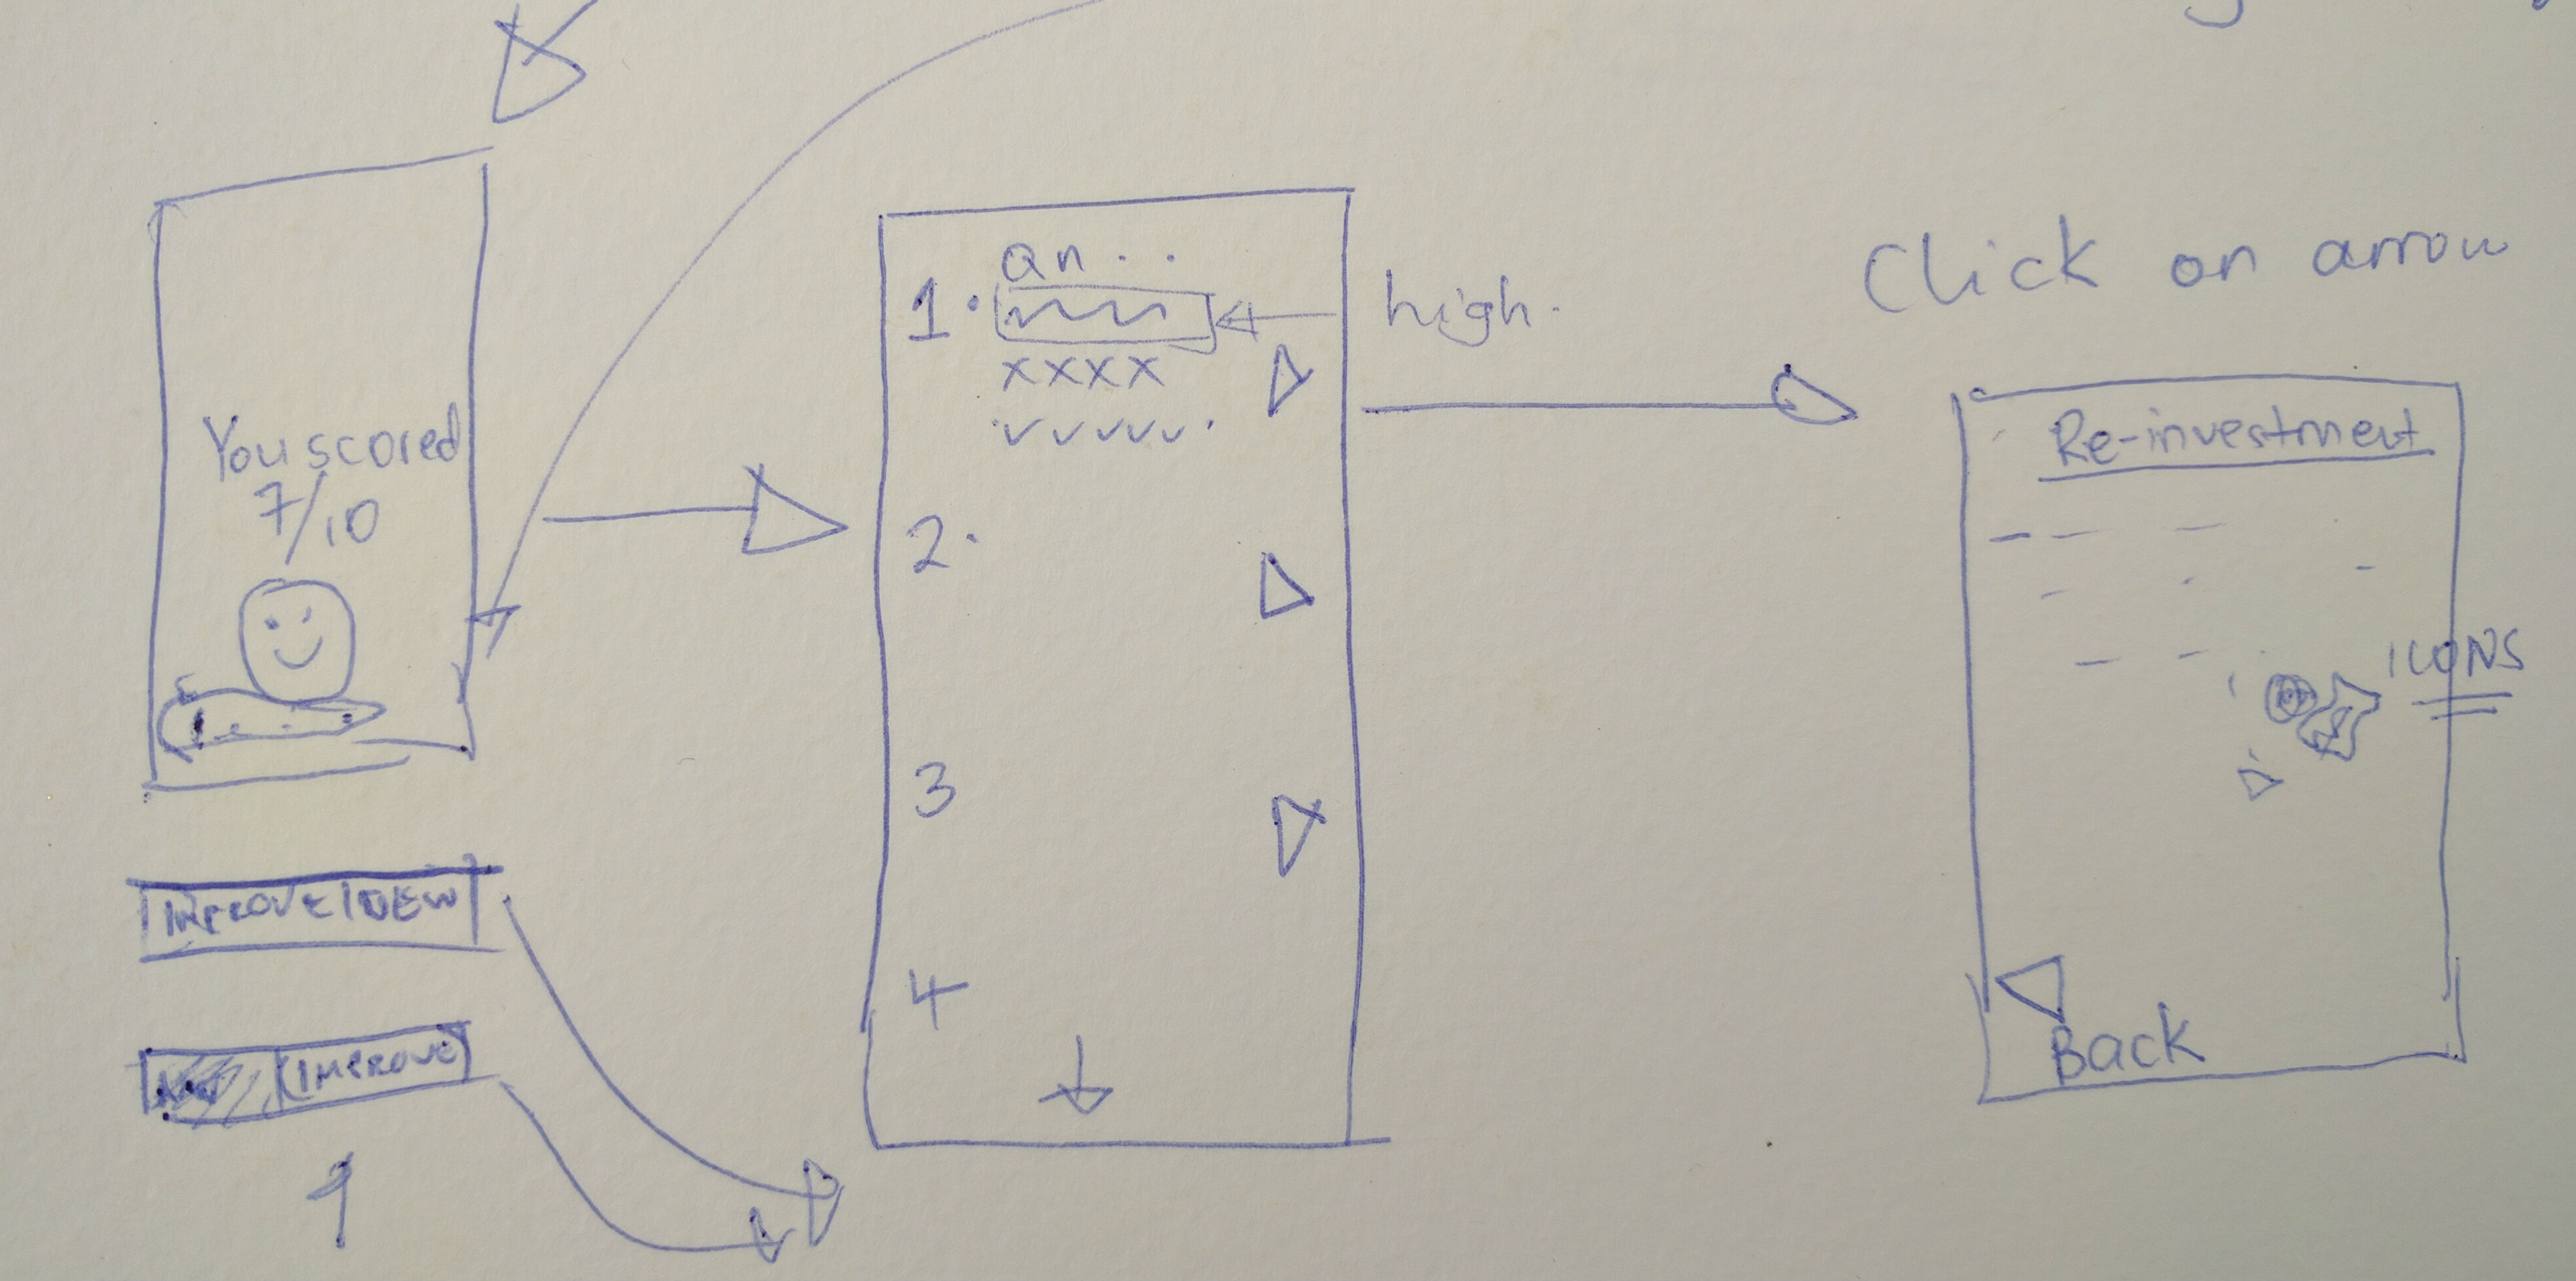
\includegraphics[width=0.8\textwidth]{biteSize.jpg}
    %IterationProcess.png
    \caption{By clicking on an arrow next to the question showing the correct answer compared to your answer, the coach could read an extract from the YoungDrive manuals, which includes the right answer. The learning benefit compared to just observing the right answer, is that the coach gets the answer in context, which improves memorization and understanding. An idea would be to no longer give the coach the correct answer in the score board, but to instead let the coach choose the right answer after reading the text.}
    \label{fig:bite-size}
\end{figure}

A major opportunity doing this would be to replace the paper manuals. Today, the manuals are the most expensive post of YoungDrive, which is why this would be attractive. While a smartphone or tablet could be returned after a YoungDrive program has ended, this is not possible with the paper versions, so there might be a monetary incentive to do so. A problem that would need to be addressed is that the manuals also have written exercises in them. These exercises could be made interactive in the app, which would also allow for smart features such as automatic assessment, financial literacy simulations, etcetera. While this was not a scope of the master thesis, it is interesting further work to test if such interactive exercises and simulations would be effective in the developing country context of learning and teaching entrepreneurship.


\subsection{Research question 5}
\subsubsection{\#5 Educator Dashboard}
Josefina has no means of accessing live quiz results today, as there is no educator dashboard developed. Instead, quiz results today needs to be transferred from a database into Google Sheets, which is cumbersome and not user-friendly.

There was not enought time to develop an educator dashboard, even if this had been a goal. Instead, low-fi trigger material was created, and co-creation stakeholder workshops were held, both for iteration 3 and 4.

In the future, this will be a must-have, and it ties well into YoungDrive's future wish of strengthening its quality assurance via monitoring and evaluation.

How powerful the educator dashboard should be might be a ethical discussion, where one could argue that me as a developer needs to be sensitive if I want the app to support the coaches to become better, and not be a tool for the project partner to fire coaches that doesn't have the same quiz results as others. As the combination of "Are you sure?" and correctness can give insight into the attitudes and care of the coaches, carefulness must be taken.

 %då Expedition Mondial ifrågasatte "Visst är väl även Christine och Patrick?" målgrupp för detta? Och vad har de för utrustning? Christine har mobil, Patrick ingen. Så detta talade för att Educator Dashboard skulle behöva fungera på mobil, och inte bara dator som jag tänkt, iom att Josefina har dator.

%Då bestämdes med Expedition Mondial att jag skulle ha workshop med dem på onsdag. Med samtal med Josefina, sade hon att de garanterat borde utrustas med tablets då de samlar in data digitalt, så jag kan tänka mig att de får en tablet framöver. Skönt! Detta stämmer även med vad Stefan FalkBoman hade tänkt sig, och de iPads han köpt in till mig. Så då kunde jag ha dessa som tanke att utforma educator-app-dashboarden ifrån.


